
\documentclass[a4paper]{article}
\usepackage[english]{babel}
\usepackage[utf8]{inputenc}
\usepackage{amsmath}
\usepackage{graphicx}
\usepackage[colorinlistoftodos]{todonotes}
\usepackage{amsmath,amssymb}
\usepackage[autostyle]{csquotes}
\usepackage{longtable}
\usepackage[singlelinecheck=off]{caption}

% adjust caption style
\usepackage[aboveskip=1pt,labelfont=bf,labelsep=period,singlelinecheck=off]{caption}
% define custom colors (this one is for figure captions)
\definecolor{Gray}{gray}{.25}

\usepackage[backend=biber,style=nature,sorting=none, citestyle=numeric]{biblatex}
\addbibresource{refs.bib}

\title{\textbf{Technical Appendix}\\
Transmission model of syphilis in Louisiana and Massachusetts\\}
\author{}
\date{}

\begin{document}
\maketitle



\section{Model overview}
\label{sec:introduction}
We constructed a deterministic compartmental model describing syphilis transmission. The model was parameterized to describe the epidemiology of syphilis in two states: Louisiana and Massachusetts. These two states both experience a high burden of disease but display different epidemic characteristics in terms of the distribution of cases by MSM status and race/ethnicity. The population was divided into compartments representing the following states: susceptible ($S$), incubating ($E$), primary syphilis ($I_1$), secondary syphilis ($I_2$), early latent syphilis ($L_1$) and late latent syphilis ($L_2$) (Figure \ref{FigS1}). In the absence of treatment, infected individuals remained in the late latent stage of infection. With treatment, individuals entered a treated state ($T_1$ - $T_3$). After treatment, individuals entered a re-susceptible ($SR$) state. A parallel set of infection stages ($ER$, $IR_1$, $IR_2$, $LR_1$, $LR_2$) were included for individuals experiencing a repeat infection. Although natural history parameters were not different for those with repeat infections compared to those with a first infection, this approach allowed us to evaluate interventions focused in a subset of the population experiencing a prior syphilis infection. We began tracking those with a prior treated infection 5 years before the start of the calibration period. The rate of exit from the treated state depended on infection stage at treatment.  The model also included a never sexually active (A) compartment. The model was stratified by sex (male and female), sexual activity group (low and high), age category (20-44 y and 45-65 y), and subpopulation. The five subpopulations were: (i) heterosexual non-Hispanic blacks, (2) heterosexual Hispanics, (iii) heterosexual ‘others’ (non-Hispanic non-black population), (iv) HIV-negative men who have sex with men (MSM), and (v) HIV-positive MSM. 

\setcounter{figure}{0}
\renewcommand{\thefigure}{S\arabic{figure}}
\begin{figure}[ht] %s state preferences regarding figure placement here
% use to correct figure counter if necessary
%\renewcommand{\thefigure}{2}

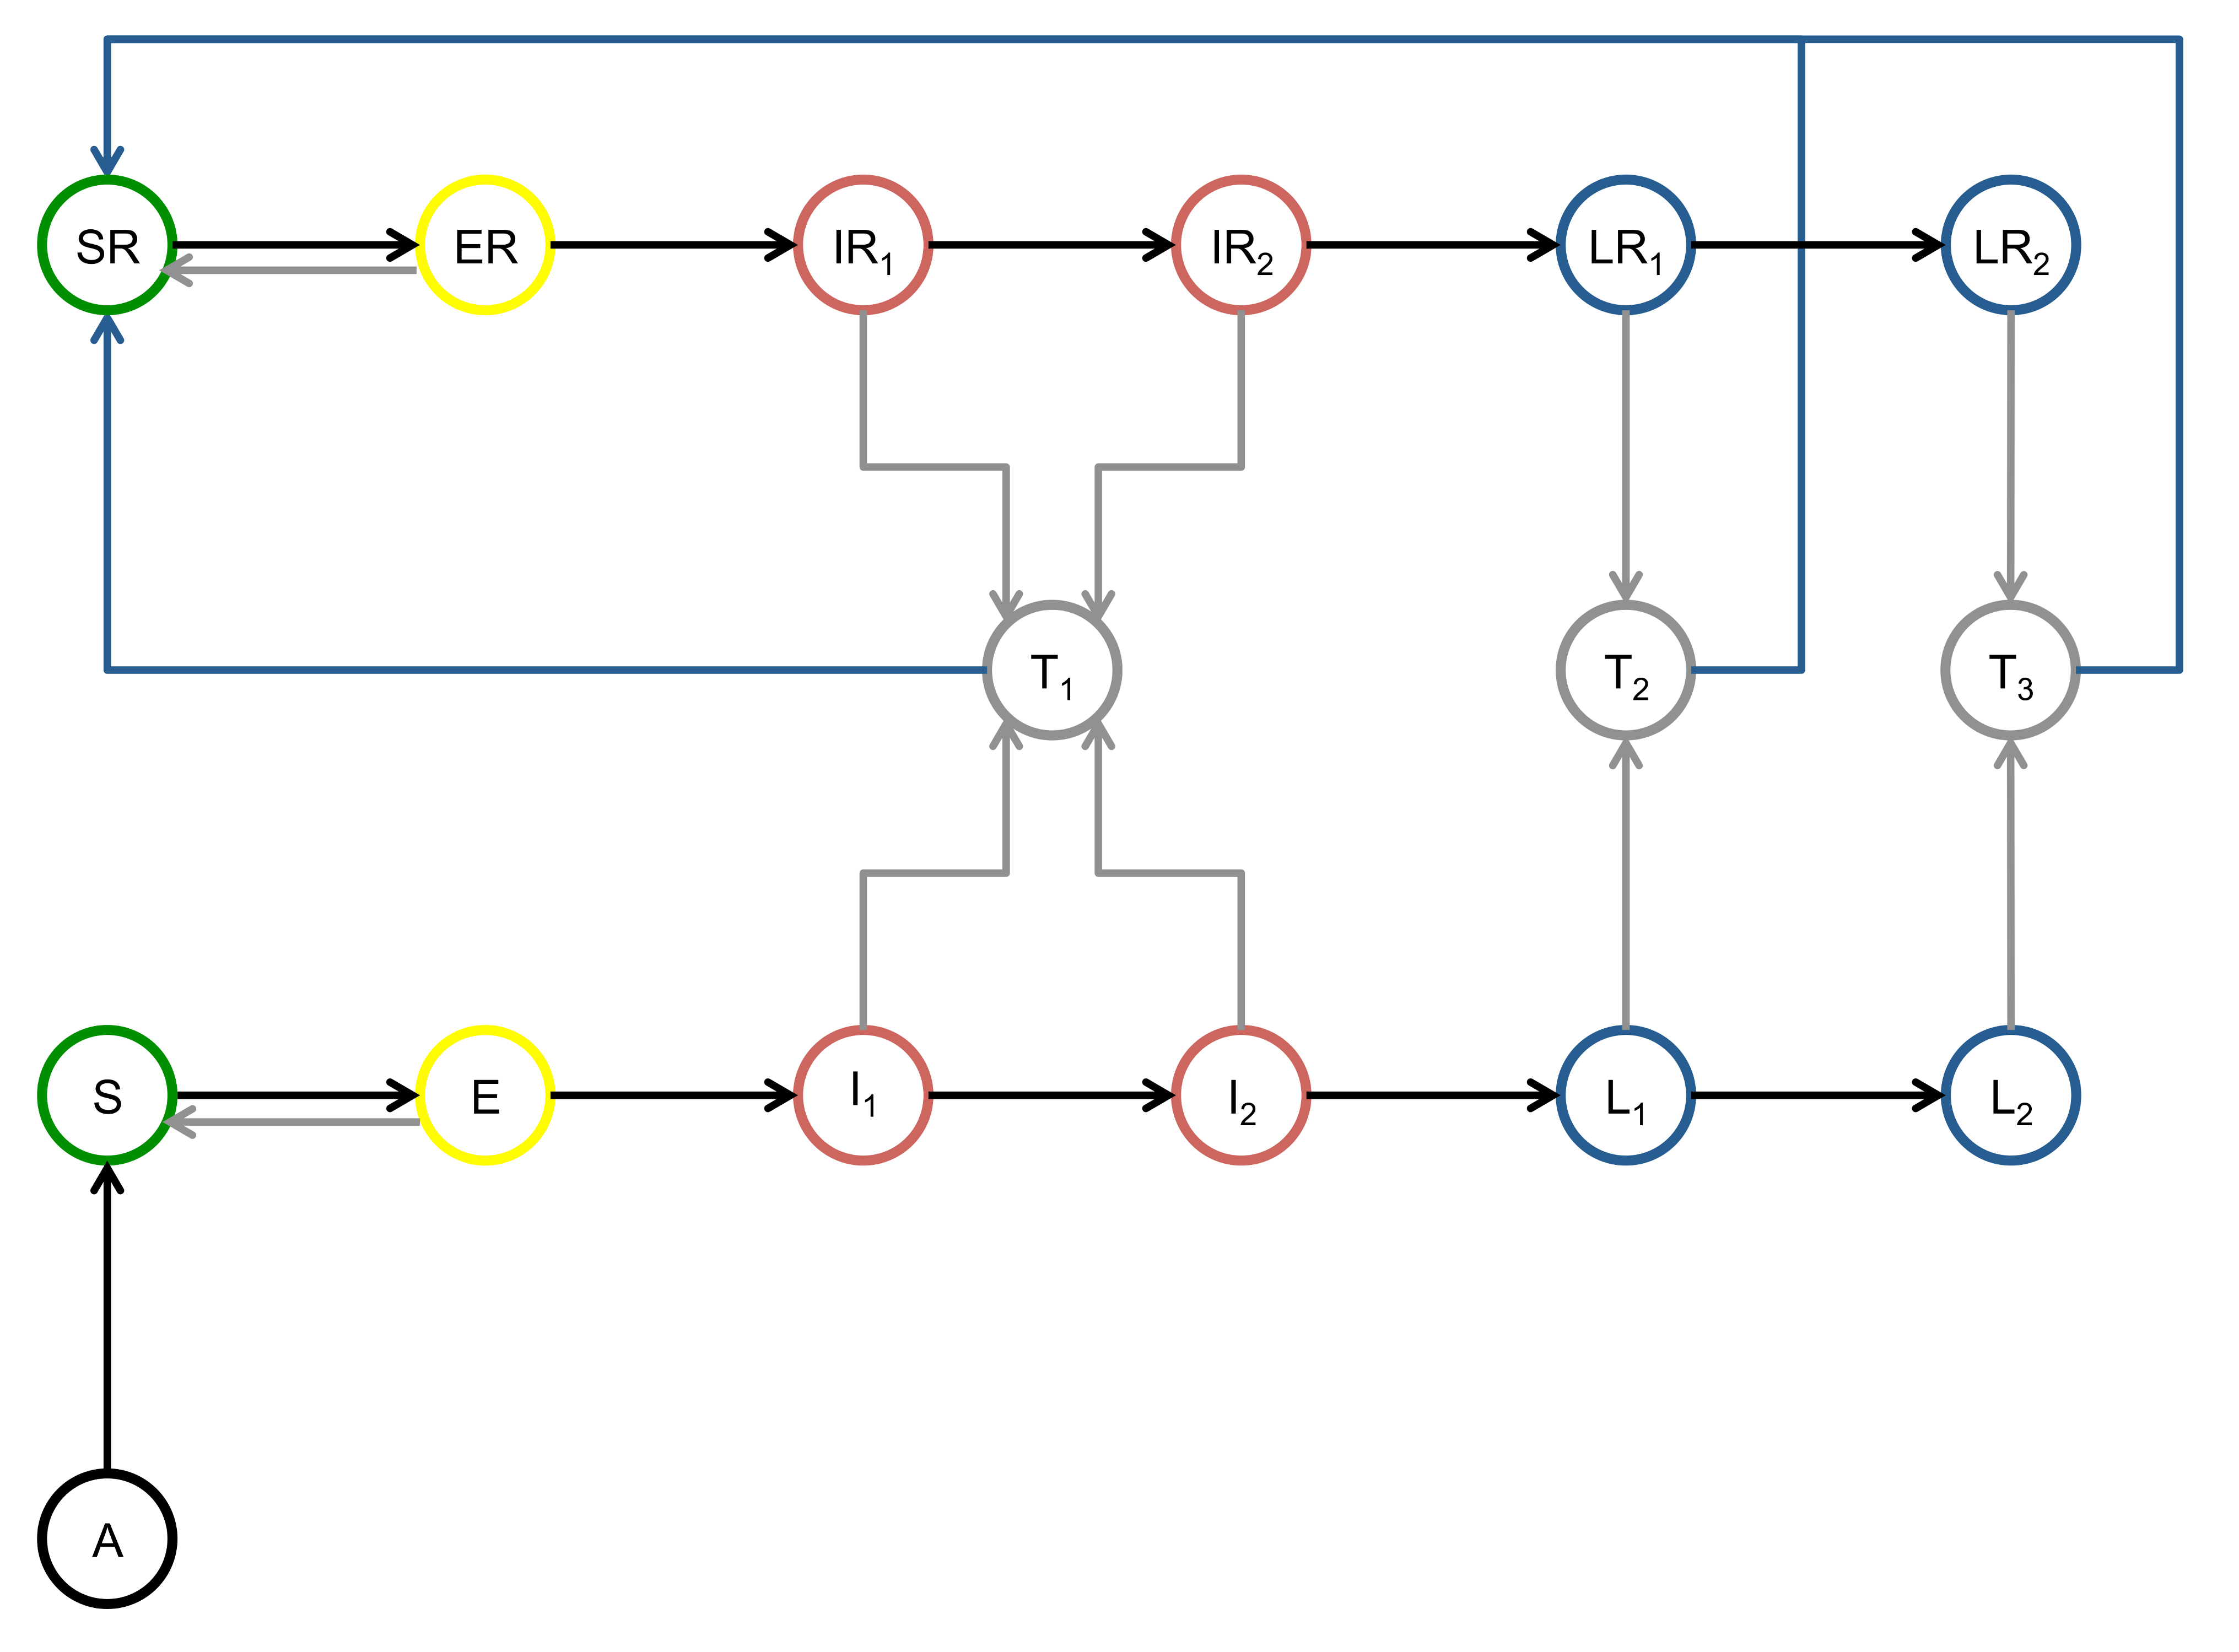
\includegraphics[width=\textwidth]{F1.png}

\caption{\color{Gray} \textbf{Syphilis transmission model overview}.}

\label{FigS1} 
\end{figure}

The proportion of the population in each racial/ethnic group was based on 2015 U.S. Census estimates~\autocite{NationalCenterforHealthStatistics.} for the states of Louisiana and Massachusetts. The proportion of males in the MSM group for each state was based on a recent analysis~\autocite{Grey2016}. We assumed an equal number of males and females; because a proportion of males were allocated to the MSM subpopulations, there were more heterosexual females than heterosexual males in the model. The age-specific prevalences of HIV in MSM were based on 2015 estimates from the Louisiana Department of Public Health and the Massachusetts Department of Public Health. For simplicity, we assumed a constant population size and a closed population; that is, no sexual partnerships occurred with individuals outside of the modeled population. New individuals entered the 20-44 year old age group in the susceptible state, with a proportion allocated to the never sexually active group, where they were not at risk of infection. As individuals aged into the older age category, a proportion of never sexually active individuals transitioned out of this compartment and were susceptible to gonorrhea infection. 

\section{Model equations and parameters}
\label{sec:eqn}
For an individual of a given subpopulation (\textit{i}), sex (\textit{j}), sexual activity group (\textit{k}), and age group (\textit{l}), the model is described by the following system of differential equations, where $N_{ijkl}$ represents the total sexually active population in a given group. Model states are provided in Table \ref{states}, and parameter definitions are presented in Table \ref{params} of this appendix. Parameter values used in the model are provided in the main text.  Details on the calculation of the sexual mixing matrix and force of infection are provided in the subsequent sections.\newline \newline
For age category 1:
\begin{equation*}\label{agecat1-1}
\begin{aligned}
  \frac{dA_{ijk1}}{dt}={} & (1-p_{s_{ijk1}} )\mu_2 (N_{ijk2} + A_{ijk2})  - \mu_1 A_{ijk1} 
    \\&\\
 \frac{dS_{ijk1}}{dt}={} & -\lambda_{ijk1} S_{ijk1}  + \phi E_{ijk1}  
 + p_{s_{ijk1}} \mu_2(N_{ijk2} + A_{ijk2}) - \mu_1 S_{ijk1}
  \\&\\
  \frac{dE_{ijk1}}{dt}={} & \lambda_{ijk1} S_{ijk1}  - \delta E_{ijk1} -\phi E_{ijkl} -\mu_1 E_{ijk1}
     \\&\\
  \frac{dI_{1_{ijk1}}}{dt}={} & \delta E_{ijk1} - \gamma_p I_{1_{ijk1}} - \tau_p I_{1_{ijk1}} - \alpha_{ijk1} I_{1_{ijk1}} -\phi I_{1_{ijk1}}  - \mu_1 I_{1_{ijk1}}
   \\&\\
  \frac{dI_{2_{ijk1}}}{dt}={} & \gamma_p I_{1_{ijk1}} - \gamma_s I_{2_{ijk1}} - \tau_s I_{2_{ijk1}} - \alpha_{ijk1} I_{2_{ijk1}} -\phi I_{2_{ijk1}}  - \mu_1 I_{2_{ijk1}}
     \\&\\
   \frac{dL_{1_{ijk1}}}{dt}={} & \gamma_s I_{2_{ijk1}} - \gamma_e L_{1_{ijk1}} - \tau_e L_{1_{ijk1}} - \alpha_{ijk1} L_{1_{ijk1}} -\phi L_{1_{ijk1}}  - \mu_1 L_{1_{ijk1}}
     \\&\\
    \frac{dL_{2_{ijk1}}}{dt}={} & \gamma_e L_{1_{ijk1}} - \tau_l L_{2_{ijk1}} - \alpha_{ijk1} L_{2_{ijk1}} -\phi L_{2_{ijk1}}   - \mu_1 L_{2_{ijk1}}
      \\&\\
    \frac{dT_{1_{ijk1}}}{dt}={} & \tau_p (I_{1_{ijk1}} + IR_{1_{ijk1}} ) + \tau_s (I_{2_{ijk1}} + IR_{2_{ijk1}}  ) + \\
    & \alpha_{ijk1} (I_{1_{ijk1}} + IR_{1_{ijk1}} + I_{2_{ijk1}} + IR_{2_{ijk1}}) + \\
    & \phi (I_{1_{ijk1}} + IR_{1_{ijk1}} + I_{2_{ijk1}} + IR_{2_{ijk1}}) - \\ 
    & \xi_{ps} T_{1_{ijk1}} - \mu_1 T_{1_{ijk1}}
     \\&\\
    \frac{dT_{2_{ijk1}}}{dt}={} & \tau_e (L_{1_{ijk1}} + LR_{1_{ijk1}} )  + \alpha_{ijk1} (L_{1_{ijk1}} + LR_{1_{ijk1}} ) + \phi (L_{1_{ijk1}} + LR_{1_{ijk1}} ) - \\
    & \xi_e T_{2_{ijk1}} - \mu_1 T_{2_{ijk1}}
     \\&\\
    \frac{dT_{3_{ijk1}}}{dt}={} & \tau_l (L_{2_{ijk1}} + LR_{2_{ijk1}}  ) + \alpha_{ijk1} (L_{2_{ijk1}} + LR_{2_{ijk1}} ) + \phi (L_{2_{ijk1}} + LR_{2_{ijk1}} ) - \\
    & \xi_l T_{3_{ijk1}} - \mu_1 T_{3_{ijk1}}
 \end{aligned}
 	\end{equation*}
 
 \begin{equation*}\label{agecat1-2}
	\begin{aligned}
          \frac{dSR_{ijk1}}{dt}={} & -\lambda_{ijk1} SR_{ijk1} + \phi ER_{ijk1} + \xi_{ps} T_{1_{ijk1}} + \xi_e T_{2_{ijk1}} + \xi_l T_{3_{ijk1}}  - \mu_1 SR_{ijk1}
   \\&\\
    \frac{dER_{ijk1}}{dt}={} & \lambda_{ijk1} SR_{ijk1} - \delta ER_{ijk1} -\phi ER_{ijk1} - \mu_1 ER_{ijk1}
     \\&\\
  \frac{dIR_{1_{ijk1}}}{dt}={} & \delta ER_{ijk1} - \gamma_p IR_{1_{ijk1}} - \tau_p IR_{1_{ijk1}} - \alpha_{ijk1} IR_{1_{ijk1}} -\phi IR_{1_{ijk1}}   - \mu_1 IR_{1_{ijk1}}
   \\&\\
  \frac{dIR_{2_{ijk1}}}{dt}={} & \gamma_p IR_{1_{ijk1}} - \gamma_s IR_{2_{ijk1}} - \tau_s IR_{2_{ijk1}} - \alpha_{ijk1} IR_{2_{ijk1}} -\phi IR_{2_{ijk1}}   - \mu_1 IR_{2_{ijk1}}
     \\&\\
   \frac{dLR_{1_{ijk1}}}{dt}={} & \gamma_s IR_{2_{ijk1}} - \gamma_e LR_{1_{ijk1}} - \tau_e LR_{1_{ijk1}} - \alpha_{ijk1} LR_{1_{ijk1}} - \phi LR_{1_{ijk1}}   - \mu_1 LR_{1_{ijk1}}
     \\&\\
    \frac{dLR_{2_{ijk1}}}{dt}={} & \gamma_e LR_{1_{ijk1}} - \tau_l LR_{2_{ijk1}} - \alpha_{ijk1} LR_{2_{ijk1}} -\phi LR_{1_{ijk1}}   - \mu_1 LR_{2_{ijk1}}
 \end{aligned}
 \end{equation*}
\\ 
For age category 2:
 \begin{equation*}\label{agecat2-1}
 \begin{aligned}
 	\frac{dA_{ijk2}}{dt}={} & (1-p_{s_{ijk2}} )\mu_1 A_{ijk1}  - \mu_2 A_{ijk2} 
     \\&\\
    \frac{dS_{ijk2}}{dt}={} & -\lambda_{ijk2} S_{ijk2} + \phi E_{ijk2} + \mu_1 S_{ijk1} + p_{s_{ijk2}} \mu_1 A_{ijk1} - \mu_2 S_{ijk2}
 \\&\\
  \frac{dE_{ijk2}}{dt}={} & \lambda_{ijk2} S_{ijk2} - \delta E_{ijk2} -\phi E_{ijk2} - \mu_2 E_{ijk2} +  \mu_1 E_{ijk2}
     \\&\\
  \frac{dI_{1_{ijk2}}}{dt}={} & \delta E_{ijk2} - \gamma_p I_{1_{ijk2}} - \tau_p I_{1_{ijk2}} - \alpha_{ijk2} I_{1_{ijk2}} -\phi  I_{1_{ijk2}} - \mu_2 I_{1_{ijk2}} + \mu_1 I_{1_{ijk1}}
   \\&\\
  \frac{dI_{2_{ijk2}}}{dt}={} & \gamma_p I_{1_{ijk2}} - \gamma_s I_{2_{ijk2}} - \tau_s I_{2_{ijk2}} - \alpha_{ijk2} I_{2_{ijk2}} -\phi I_{2_{ijk2}} - \mu_2 I_{2_{ijk2}} + \mu_1 I_{2_{ijk1}}
     \\&\\
   \frac{dL_{1_{ijk2}}}{dt}={} & \gamma_s I_{2_{ijk2}} - \gamma_e L_{1_{ijk2}} - \tau_e L_{1_{ijk2}} - \alpha_{ijk2} L_{1_{ijk2}} -phi L_{1_{ijk2}}  - \mu_2 L_{1_{ijk2}} + \mu_1 L_{1_{ijk1}}
     \\&\\
    \frac{dL_{2_{ijk2}}}{dt}={} & \gamma_e L_{1_{ijk2}} - \tau_l L_{2_{ijk2}} - \alpha_{ijk2} L_{2_{ijk2}} - \phi L_{2_{ijk2}}  - \mu_2 L_{2_{ijk2}} + \mu_1 L_{2_{ijk1}}
 \end{aligned}
 	\end{equation*}
 \begin{equation*}\label{agecat2-2}
 	\begin{aligned}
    \frac{dT_{1_{ijk2}}}{dt}={} & \tau_p (I_{1_{ijk2}} + IR_{1_{ijk2}} ) + \tau_s (I_{2_{ijk2}} + IR_{2_{ijk2}} ) + \\
    & \alpha_{ijk2} (I_{1_{ijk2}} + IR_{1_{ijk2}} + I_{2_{ijk2}} + IR_{2_{ijk2}}) + \\
    & \phi (I_{1_{ijk2}} + IR_{1_{ijk2}} + I_{2_{ijk2}} + IR_{2_{ijk2}}) - \\
    & \xi_{ps} T_{1_{ijk2}} - \mu_2 T_{1_{ijk2}} + \mu_1 T_{1_{ijk1}}
     \\&\\
    \frac{dT_{2_{ijk2}}}{dt}={} & \tau_e (L_{1_{ijk2}} + LR_{1_{ijk2}})  + \alpha_{ijk2} (L_{1_{ijk2}} + LR_{1_{ijk2}} ) +\phi (L_{1_{ijk2}} + LR_{1_{ijk2}} ) - \\
    & \xi_e T_{2_{ijk2}} - \mu_2 T_{2_{ijk2}} + \mu_1 T_{2_{ijk1}}
     \\&\\
    \frac{dT_{3_{ijk2}}}{dt}={} & \tau_l (L_{2_{ijk2}} + LR_{2_{ijk2}})  + \alpha_{ijk2} (L_{2_{ijk2}} + LR_{2_{ijk2}} ) +\phi (L_{2_{ijk2}} + LR_{2_{ijk2}} ) - \\
    & \xi_l T_{3_{ijk2}} - \mu_2 T_{3_{ijk2}} + \mu_1 T_{3_{ijk1}}
    \\&\\
      \frac{dSR_{ijk2}}{dt}={} & -\lambda_{ijk2} SR_{ijk2} + \phi ER_{ijk2} + \xi_{ps} T_{1_{ijk2}} + \xi_e T_{2_{ijk2}} + \xi_l T_{3_{ijk2}}  - \mu_2 SR_{ijk2} +  \mu_1 SR_{ijk1}
   \\&\\
   \frac{dER_{ijk2}}{dt}={} & \lambda_{ijk2} SR_{ijk2} - \delta ER_{ijk2} - -\phi ER_{ijk2} \mu_2 ER_{ijk2} +  \mu_1 ER_{ijk1}
     \\&\\
  \frac{dIR_{1_{ijk2}}}{dt}={} & \delta ER_{ijk2} - \gamma_p IR_{1_{ijk2}} - \tau_p IR_{1_{ijk2}} - \alpha_{ijk2} IR_{1_{ijk2}} -\phi IR_{1_{ijk2}}  - \mu_2 IR_{1_{ijk2}} + \mu_1 IR_{1_{ijk1}}
   \\&\\
  \frac{dIR_{2_{ijk2}}}{dt}={} & \gamma_p IR_{1_{ijk2}} - \gamma_s IR_{2_{ijk2}} - \tau_s IR_{2_{ijk2}} - \alpha_{ijk2} IR_{2_{ijk2}} -\phi IR_{2_{ijk2}} - \mu_2 IR_{2_{ijk2}} + \mu_1 IR_{2_{ijk1}}
     \\&\\
   \frac{dLR_{1_{ijk2}}}{dt}={} & \gamma_s IR_{2_{ijk2}} - \gamma_e LR_{1_{ijk2}} - \tau_e LR_{1_{ijk2}} - \alpha_{ijk2} LR_{1_{ijk2}} -phi LR_{1_{ijk2}}  - \mu_2 LR_{1_{ijk2}} + \mu_1 LR_{1_{ijk1}}
     \\&\\
    \frac{dLR_{2_{ijk2}}}{dt}={} & \gamma_e LR_{1_{ijk2}} - \tau_l LR_{2_{ijk2}} - \alpha_{ijk2} LR_{2_{ijk2}} -\phi LR_{2_{ijk2}} - \mu_2 LR_{2_{ijk2}} + \mu_1 LR_{2_{ijk1}}
\end{aligned}
\end{equation*}
\newline Cumulative reported early syphilis cases (D) are calculated as:
\begin{equation*}\label{3}
	\begin{aligned}
		\frac{dD_{ijkl}}{dt}={} & \omega (\alpha_{ijkl} *(I_{1_{ijkl}} + IR_{1_{ijkl}}  + I_{2_{ijkl}} + IR_{2_{ijkl}} + L_{1_{ijkl}} +  LR_{1_{ijkl}}) + \\  
& \eta_j (\tau_p (I_{1_{ijkl}} + IR_{1_{ijkl}} ) + \tau_s (I_{2_{ijkl}} + IR_{2_{ijkl}} )  + \tau_e (L_{1_{ijkl}} + LR_{1_{ijkl}}) ) )
	\end{aligned}
\end{equation*}
\newpage
\setcounter{table}{0}
\renewcommand{\thetable}{S\arabic{table}}
\section{Model states and parameters}

\label{sec:params}
	\begin{longtable}[c]  {p{1.5cm}p{9cm}}
    \caption{Model states and definitions. \label{states}}\\
    \hline
    State & Definition\\
	\hline
    \endfirsthead
    
    \hline
    State & Definition\\
	\hline
    \endhead
    
    \hline
    \endfoot
    
    \hline
    \endlastfoot
    
    $S$	& Susceptible\\
    $E$ & Exposed (incubating and not infectious)\\
    $I_1$ & Primary syphilis\\
    $I_2$ & Secondary syphilis\\
    $L_1$ & Early latent syphilis\\
    $L_2$ & Late latent syphilis\\
    $SR$	& Susceptible, previously treated infection\\
    $ER$	& Exposed, previously treated infection\\
    $IR_1$	& Primary syphilis, previously treated infection\\
    $IR_2$	& Secondary syphilis, previously treated infection\\
    $LR_1$	& Early latent syphilis, previously treated infection\\
    $LR_2$	& Late latent syphilis, previously treated infection\\
    $T_1$ & Treated infectious syphilis\\
    $T_2$ & Treated early latent syphilis\\
    $T_3$ & Treated late latent syphilis\\
    $A$ & Never sexually active\\
     
	\end{longtable} 
\newpage
\begin{longtable}[l]   {p{1.5cm}p{9cm}}
    \caption{Parameter symbols and definitions. \label{params}}\\
    \hline
    Symbol & Definition\\
	\hline
    \endfirsthead
    
    \hline
    Symbol & Definition\\
	\hline
    \endhead
    
    \hline
    \endfoot
    
    \hline
    \endlastfoot
    
    $i$	& Subpopulation\\
    $j$	& Sex\\
    $k$	& Sexual activity group\\
    $l$	& Age group\\
    $\mu$ & Rate of exit from age group\\
    $p_s$ & Probability of entry into sexually active population\\
    $\lambda$ & Force of infection\\
    $\delta$ & 1/Average duration of exposed state\\
    $\gamma_p$ & 1/Average duration of primary infection\\
    $\gamma_s$ & 1/Average duration of secondary infection\\
    $\gamma_e$ & 1/Average duration of early latent infection\\
    $\tau_p$ & Rate of seeking medical treatment for primary syphilis\\
    $\tau_s$ & Rate of seeking medical treatment for secondary syphilis\\
    $\tau_e$ & Rate of seeking medical treatment for early latent syphilis\\
    $\tau_l$ & Rate of seeking medical treatment for late latent syphilis\\
    $\alpha$ & Screening rate\\
    $\phi$ & Background antibiotic treatment rate\\
    $\xi_{ps}$ & 1/Duration of protection from reinfection after treatment of primary or secondary syphilis\\
    $\xi_{e}$ & 1/Duration of protection from reinfection after treatment of early latent syphilis\\
    $\xi_{l}$ & 1/Duration of protection from reinfection after treatment of late latent syphilis\\
    $\omega$ & Probability case is reported\\
    $\eta$ 	 & Relative risk case is reported if symptomatic\\
	\end{longtable}  
    
\section{Entry and exit rates}
The rates of entry/exit between the two MSM subpopulations (i=4 and 5) were adjusted to account for age-dependent differences in the prevalence of HIV infection in MSM (higher in the older age group). For HIV-negative MSM, the transitions from age group 1 to 2 was calculated as:
\[\mu_1  \left( 1 - \frac{pHIV_2 - pHIV_1}{1-pHIV_1}\right)\] for MSM remaining in the HIV-negative population and: 
\[\mu_1 \left( \frac{pHIV_2 - pHIV_1}{1-pHIV_1} \right)\] for MSM transitioning to the HIV-positive population as they moved into the older age category.

Similarly, for HIV-positive MSM, the transitions from age group 2 to 1 (aging out of the model population and re-entering in the susceptible state) were calculated as: 
\[\mu_2  \left( \frac{pHIV_1}{pHIV_2}\right)\] for MSM re-entering the model in the HIV-infected subpopulation and:
\[\mu_2  \left( 1 - \frac{pHIV_1}{pHIV_2}\right)\] for MSM re-entering the model as HIV negative.    

\section{Sexual mixing}
\label{sec:mixing}

Annual minimum rates of partner acquisition ($c_{min}$) for a given age category and sex were estimated by model fitting, with estimates for MSM derived separately from other males. Prior estimates for relative rates of partner acquisition (\textit{rp}) in different population groups were estimated as described in section \ref{subsec:param}. For an individual of a given subpopulation (\textit{i}), sex (\textit{j}), sexual activity group (\textit{k}), and age group (\textit{l}), the mean annual rate of partner acquisition was calculated as:

\[c_{ijkl} = c_{min_{ijl}}rp_{ijkl}\]

The mixing matrix takes into account sexual activity group, age, and subpopulation membership. Within a given subpopulation (\textit{i}), we describe the probability that a person of sexual activity class \textit{k} and age group \textit{l} will form a partnership with a person of activity class \textit{s} and age group \textit{t} as:

\begin{equation*}\label{mixing}
\begin{aligned}
\rho_{ijklst}={} & (\epsilon_{1,i} \delta_{ks} + 
(1-\epsilon_{1,i})\frac{{\mathop{\sum\limits_{v=1}^2}} N_{ij'sv}c_{ij'sv}}{{\mathop{\sum\limits_{u=1}^2 \sum\limits_{v=1}^2}} N_{ij'uv} c_{ij'uv}})\\ & *(\epsilon_{2,ijl} \delta_{lt} + 
(1-\epsilon_{2,ijl})\frac{{\mathop{\sum\limits_{u=1}^2}} N_{ij'ut}c_{ij'ut}}{{\mathop{\sum\limits_{u=1}^2 \sum\limits_{v=1}^2}} N_{ij'uv} c_{ij'uv}})
\end{aligned}
\end{equation*}

where \(\delta_{xy} = 1\) if \(x=y\) and 0 otherwise. $\epsilon_{1,i}$ defines mixing between sexual activity groups, while $\epsilon_{2,ijl}$ defines mixing between age groups, with values ranging from 0 (random or proportionate mixing) to 1 (assortative or `like with like' mixing). Here, $j'$ indicates that a partnership is formed with an individual of the opposite sex. For partnerships within the MSM population, $j'=j$. 
A final parameter, $\epsilon_{3,ij}$, defines mixing between subpopulations; when equal to 1, all partnerships are formed with individuals belonging to the same subpopulation, and when equal to 0, all partnerships are formed with individuals from other subpopulations. For partnerships occurring outside of an individual's subpopulation, we assumed that the parameters describing age and sexual activity assortativity remained unchanged (i.e., preference for age or sexual risk group assortative mixing was the same, regardless of whether a partner was a member of the same subpopulation or not). The one exception to this assumption related to partnerships forming between MSM and females. For these partnerships, we assumed that age assortativity followed the age preferences for partnerships between females and males, rather than the age preferences for male-male partnerships. Partnerships formed outside of an individual's own subpopulation were assumed to be be distributed proportionally to the sizes of the other subpopulations. Here, \textit{m} describes the subpopulation of the partner.\bigskip

For \(i=m\),
\\
\[\rho_{ijklmst} = \epsilon_{3,ij} \rho_{ijklst}\] \bigskip

Otherwise (i.e., for \(i \ne m\) ),
\[\rho_{ijklmst} = (1- \epsilon_{3,ij})\frac{N_{mj'st}}{\mathop{\sum\limits_{w,w\ne i}^5} N_{wj'st}} \rho_{ijklst}\]

For MSM, we included a parameter ($\theta_{HIV}$) describing serosorting in MSM (preferential selection of partners with the same HIV status), which could range from 0 to 1. When $\theta_{HIV} = 1$, MSM only had sexual partners of the same HIV status.  

For $i$ = $m$ = 4 or $i$ = $m$ = 5, 

\[\rho_{ijklmst} = \theta_{HIV} \epsilon_{3, ij} \rho_{ijklst}\]

For $i$ = 4 and $m$=5 or $i$=5 and $m$ = 4 (i.e., partner is MSM of discordant HIV status), 

\[\rho_{ijklmst} = (1 - \theta_{HIV}) \epsilon_{3, ij} \rho_{ijklst}\] \bigskip

We used the approach of Garnett and Anderson~\autocite{Garnett1994} to ensure that partnerships were balanced. When balancing partnership change rates within a subpopulation, we assumed that both sexes compromised equally, such that the number of partnerships formed was equal to the arithmetic mean of the number of partners desired by each sex, and used these adjusted partner change rates ($c_{ijlkmst}$) to calculate the force of infection (below).

To balance partnerships across subpopulations, we assumed that the group with the smaller population size determined the total number of partnerships formed. For example, the partner change rate between Hispanic females and non-Hispanic non-black males was determined by the desired number of partnerships in the females, since they represented a smaller proportion of the population. 

\section{Force of infection}
\label{sec:FOI}
The rate at which susceptible individuals are infected depends on the partner change rate ($c_{ijklmst}$), the transmission probability per partnership ($\beta_{ji}$) and the sexual mixing matrix ($\rho_{ijklmst}$), where \textit{m}, \textit{s}, and \textit{t} represent the subpopulation, sexual activity group, and age category, respectively, of the sexual partner:
\[\lambda_{ijkl} = c_{rr} \beta_{ji} \sum_{m=1}^5 \sum_{s=1}^2 \sum_{t=1}^2 \frac{c_{ijklmst}\rho_{ijklmst}(I_{1_{mj'st}}+IR_{1_{mj'st}} + I_{2_{mj'st}}+IR_{2_{mj'st}})}{N_{mj'st}}\] 

Note that \textit{j'} indicates a partnership that is formed with an individual of the opposite sex. For partnerships formed within the MSM subpopulations, \({j'}=j\). For heterosexual males, no partnerships are formed with MSM. $c_{rr}$ is a time-varying term (estimated via model calibration) that represents relative risk of transmission in MSM, to account for changes in sexual risk behaviors over time; this parameter was assumed to be 1 in all other subpopulations. 

\section{Model calibration and parameterization}
\subsection{Calibration}
\label{subsec:calibration}

We calibrated parameters describing sexual mixing, syphilis natural history, and screening and treatment rates using an adaptive Metropolis-Hastings MCMC algorithm implemented in R~\autocite{Camacho2016}. This method uses a Bayesian approach to estimate probability distributions for uncertain parameters, given the model and available data. The adaptive procedure works to optimize the proposal distribution by first adapting the size of the covariance matrix to achieve an optimal acceptance rate, and then adapting the shape of the covariance matrix~\autocite{Camacho2015}. The model calibration process was performed separately for the models describing syphilis transmission in Louisiana and Massachusetts.

Prior parameter distributions were guided by the available data, using point estimates and plausible ranges obtained from the biomedical literature where possible, or based on expert opinion or assumption, as described in Tables 1 and 2 of the main text. When information about parameters was scarce (e.g., sexual mixing coefficients), we assumed broad priors. We used the rriskDistributions package~\autocite{Belgorodski2016} to estimate the parameters describing the prior probability distribution functions. Time-varying parameters (reporting probabilities and screening rates) were described by cubic Bézier curves, a type of parametric curve that allows for a sufficient degree of flexibility in the possible shapes it can take without requiring a large number of parameters to define it (described in more detail in \ref{subsubsec:bezier}). Parameters were either log transformed (to ensure positivity) or logit transformed (to ensure probabilities were bounded between 0 and 1). Additional details on model parameterization and calibration data targets are provided below.

The likelihood was specified as beta distributions around estimates of proportion of reported early syphilis male cases occurring in MSM, proportion of reported early syphilis cases in MSM with HIV co-infection, and proportion of early syphilis cases diagnosed in the secondary or early latent stages, and normal distributions for reported rates of early syphilis and relative reporting rates for early syphilis in black and Hispanic cases (data sources described in \ref{subsec:data}). Error variance was estimated from the data. For the diagnosed case data, we assumed 95\% confidence intervals of $+/-$ 20\% of the point estimates. 

We used 10 independent MCMC chains of 100,000 iterations. These chains were visually assessed to ensure convergence and combined after burning and thinning. The prior and posterior distributions of the model parameters are presented in Figure \textbf{SX} and the results of model fitting are shown in \textbf{Figure X} and \textbf{Figure SX2}. 

\subsection{Parameters}
\subsubsection{Sexual mixing parameters}
\label{subsec:param}
The model included parameters describing assortativity of sexual mixing by age, sexual activity group, and subpopulation, which were used to calculate the sexual mixing matrix~\autocite{Garnett1994}. For the heterosexual populations, all partnerships occurred with the opposite sex. For MSM, all within subpopulation mixing was with males, with bridging events occurring via sexual partnerships with females in the other subpopulations. 

Estimates of prior values for relative rates of partner acquisition (\textit{rp}) in individuals aged 20-44 y were informed by 2011-2013 National Survey of Family Growth estimates of reported lifetime sexual partners at the national level~\autocite{U.S.DepartmentofHealthandHumanServices}. For a given racial/ethnic group, individuals in the $90^{th}$ percentile of lifetime partners were assigned to the high sexual activity group, with the remainder of the population allocated to the low sexual activity group. We excluded individuals who reported no sexual partners in their lifetime. As the survey data are capped at a maximum of 50 lifetime partners, we fit censored log normal distributions to derive estimates of the median number of lifetime partners in the high and low activity groups. We used these values to estimate relative rates of partner change by sexual activity group and subpopulation for a given sex. 

We also used estimates of mixing across age groups and subpopulations from the 2011-2013 NSFG~\autocite{U.S.DepartmentofHealthandHumanServices} for individuals aged 20-44 y. The reported race/ethnicity of respondents’ most recent sexual partner was used to estimate assortativity within subpopulations, with proportions stratified by sex. For sexually active survey respondents we obtained estimates of the proportion of most recent sexual partners that belonged to the same age category as the respondent by sex. 

We did not observe significant differences across race/ethnicity in the proportion of respondents reporting age-assortative partners. As comparable measures were not available for MSM respondents and individuals aged $\ge 45$ y, we used assumption to inform model priors describing sexual mixing in these groups. 

\subsubsection{Natural history parameters}
\label{subsec:nat hist}
Parameters describing the natural history of syphilis were based primarily on a review of existing literature~\autocite{Garnett1997}. We allowed for the possibility of a period of protection from re-infection following receipt of treatment ($\xi$). The immune period was assumed to be short (7-21 days) following treatment for primary and secondary syphilis ($\xi_{ps}$). We assumed the period of protective immunity following treatment for early latent infection ($\xi_e$) was equal to or longer than the duration for treated primary or secondary syphilis. This was implemented in the model by multiplying the duration of protective immunity following treatment of primary or secondary syphilis ($\xi_{ps}$) by a multiplier ($rr_{imm}$) that was allowed to range from 1-10, giving a possible prior for duration of immunity ($\xi_e$) of 7-210 days. Estimates of duration of immunity following treatment of late latent syphilis ($\xi_l$) had a wide prior associated with it, with the 95\% credible interval spanning 30 days to 5 years. 
\subsubsection{Time-varying parameters}
\label{subsubsec:bezier}
Screening rates and reporting probabilities were modeled as time-varying parameters, described by cubic B\'ezier curves. Each curve is defined by a start point ($P_0$), end point ($P_3$), and two internal control points ($P_1$ and $P_2$). 
\[Y(t) = (1-t)^3 P_0 + 3(1-t)^2 t P_1 + 3(1-t) t^2 P_2 + t^3 P_3\]

We used a cubic B\'ezier interpolation to reparameterize the function to produce a smooth curve going through 4 equally spaced points ($y_0$, $y_1$, $y_2$, $y_3$). The start and end points represent the values of screening/reporting at the beginning and end of the calibration period, respectively, while the two internal points determine the shape of the curve between the start and end points. Priors for the start and end points are provided in Table 2 of the main text. The two internal points were parameterized to fall between the start and end points:
\begin{equation*}\label{4}
\begin{aligned}
y_1 = {} & y_0 + (y_3 - y_0) Beta(1,1) \\
y_2 = {} & y_1 + (y_3 - y_1) Beta(1,1) \\
\end{aligned}
\end{equation*}

The Beta(1,1) distribution provided a broad prior, with the 95\% interval spanning 0.025-0.975. These parameters were rescaled to control points for the B\'ezier function as: 
\begin{equation*}\label{5}
\begin{aligned}
P_0 = {} & y_0 \\
P_1 = {} & (-5 y_0 +18 y_1 - 9 y_2 + 2 y_3)/6\\
P_2 = {} & (2 y_0 -9 y_1 + 18 y_2 - 5 y_3)/6\\
P_3 = {} & y_3 \\
\end{aligned}
\end{equation*}

These points were entered into the original cubic B\'ezier function to calculate the screening/reporting rate at each desired time point. The start point of the time-varying parameters was assumed to occur 10 years prior to the calibration period start in 2012 to prevent unrealistically abrupt changes in screening or reporting. 

To limit the number of time-varying parameters estimated by model calibration, we assumed that the screening rates and reporting probabilities in some groups followed the same shape as those estimated as described above, but had different magnitudes. This was implemented by multiplying these time-varying parameters by relative risks for specific population groups, as presented in \textbf{Table 2}. Specifically, reporting probabilities in cases actively seeking medical care were calculated as:
\[\omega * \eta_j\] with $\eta_j$ representing the relative risk a case is reported if symptomatic and $\omega$ representing the time-varying reporting probability for cases identified by screening. 

Screening rates ($\alpha_{ijkl}$) were calculated as: 
\[ \psi_{ij} * rr_{ac_{k}} *  rr_{pop_{ij}} * rr_{age_{i}} \] where $rr_{ac_{k}}$ is the relative risk of screening by sexual activity group, $rr_{pop_{ij}}$ is the relative risk of screening by subpopulation and sex,  $rr_{age_{i}}$ is the relative risk of screening by subpopulation, and $\psi_{ij}$ is the time-varying estimate of annual screening rate for the low sexual activity group of a given sex and subpopulation.  

Background antibiotic treatment was included in the model to capture the effect of penicillin on reducing syphilis burden in the population. We allowed for relatively high rates of treatment (15\% per year) for a 40-year period that stopped 20 years before the calibration period started. After this, background treatment was continued at a rate of 1\% per year. These would represent cases receiving treatment for another reason that resulted in inadvertent treatment of their syphilis infection. These treated cases would not be counted among reported cases.
\subsection{Data for model calibration}
\label{subsec:data}

Annual data on syphilis reported cases were used to ensure our model was reproducing observed trends. We used data collected by the Louisiana Department of Public Health and the Massachusetts Department of Public Health for the years 2012-2016. The model was fit separately to data from Louisiana and Massachusetts. In addition to overall rates of diagnosed early (primary, secondary, and early latent) syphilis by age and sex, we also used data on the stage at which cases were diagnosed for model fitting (proportion of all early early syphilis cases that were diagnosed as secondary or early latent by year). Given the low overall number of early syphilis cases reported in females aged 45-64y, we did not use the stage at diagnosis calibration target in this age group. For each sex and age group, we calculated relative diagnosis rates of early syphilis in non-Hispanic black and Hispanic populations, using overall rates as the referent. For calibration purposes, we used the mean value of these rate ratios over the 5-year period, with the minimum and maximum value assumed to represented the 95\% intervals of the data. Estimates of proportion of male cases identified as MSM and proportion of MSM cases with HIV co-infection were used as additional model calibration targets. Data on HIV co-infection in MSM were limited to the years 2014-2016 for Louisiana. Finally, we used state-level estimates of the proportion of all reported syphilis cases (including late latent) that were diagnosed in the primary, secondary, or early latent stage~\autocite{cdc2017}. We used average values for the years 2012-2016. Note that these data were for all cases, and were not limited to the model age groups. 

\newpage
\printbibliography 
\end{document}
